\newpage
\subsection{Framework}\label{subsec: Framework}

\subsubsection{Entwicklerumgebung} 
\begin{figure}[H]
	\centering
	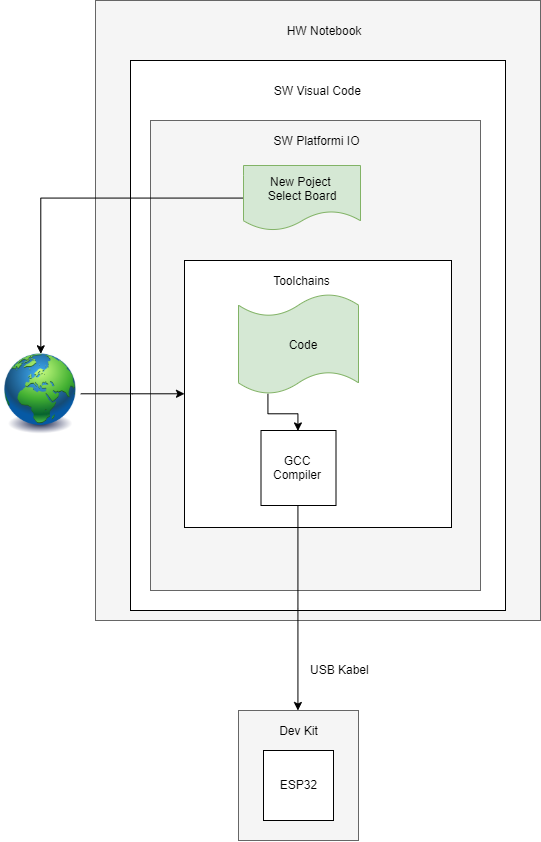
\includegraphics[width=0.8\textwidth]{graphics/DevelopDiagram.png}
	\caption{Entwicklungs Umgebung}
	\label{pic: PIO}
\end{figure} 

 Als Entwicklungsumgebung wird Visual Code von der Firma Microsoft verwendet, dies ist ein freier Quelltext-Editor, mit dem unter anderem Debugging möglich ist \cite{noauthor_visual_nodate}. In Visual Code können Extensions eingebunden werden, somit wird PlatformIO IDE \cite{platformio_platformio_nodate} kurz PIO Installiert und Openhab.
PIO ist ein plattformübergreifender Code Builder und Bibliotheksmanger. Wird ein neues Projekt eröffnet, muss vom Benutzer zuerst das Entwickler Board gewählt werden, anschliessend kümmert sich PIO um die erforderlichen Toolchains, ladet diese vom Internet herunter und installiert sie. Nun kann das Developmend-Board via USB Kabel angesprochen werden. Programmcode kann kompiliert und auf den Mikrocontroller geladen werden, die Serial Port ausgaben können direkt im PIO angezeigt werden. In Abbildung \ref{pic: PIO} ist ein Blockdiagramm auf dem die Verbindungen zwischen Software und Hardware dargestellt sind.

\subsubsection{Framework Arduino}
In dem Arduino Framework erfolgt die Programmierung in C und in C++ . Das Arduino Framework steht unter der LGPL/GPL Lizenz und ist somit eine freie Software. Ein grosser Vorteil des Arduino Frameworks ist, dass zahlreiche Bibliotheken und sowie Programmcode auf  Github erhältlich sind \cite{noauthor_arduino_nodate}.Die Wahl des Arduino Framwork ist auf Grund der Programmiersprache, Verfügbarkeit und bisherigen Erfahrungen erfolgt. Ein Funktionsmuster mit Hotspot, für Grundkonfigurationen und erste MQTT-Nachrichten, konnten Erfolgreich mit dem Arduino Framework realisiert werden.

\subsubsection{Smart-Home Plattform Openhab}
\label{subsubsec: Smart-Home Plattform}
Eine Smart-Home Plattform wird benötigt, damit der Benutzer mit dem IOT-Systems interagieren kann. 
Mit der Openhab Smart-Home-Plattform sind folgende Bedingungen erfüllt:\\
\begin{enumerate}
	\item Bietet Schnittstellen mit anderen Smart-Home Technologien wie KNX
	\item Benutzerfreundlich
	\item Client einsetzbar mittels verschiedenen Betriebssystemen
	\item Unabhängig vom öffentlichen Netz (Inhouse Server) 
\end{enumerate}
Openhab bietet sehr viele Schnittstellen, da durch den modularen Aufbau der Architektur die flexible Anbindung neuer Technologien einfach ist. Die für dieses Projekt wichtige Bindings von MQTT-Broker und KNX sind somit vorhanden. Was ebenso interessant ist, sind konfigurierbare Features wie Dropbox Support, und Google Kalender.